\documentclass{article}
\usepackage{amsmath}
\usepackage{geometry}
\usepackage{graphicx}
\usepackage{tikz}
\usetikzlibrary{graphs, graphs.standard}
\geometry{a4paper, margin=1in}

\title{Chip Firing Graphs}
\author{Implementation Notes}
\date{\today}

\begin{document}

\maketitle

\section{Introduction}
This document outlines the mathematical formulation of chip firing graphs implemented in the library.

\section{Definitions}
Let $G = (V, E)$ be an undirected graph with vertices $V = \{v_1, v_2, \ldots, v_n\}$ and edges $E \subseteq V \times V$.

A \textbf{chip configuration} on $G$ is a vector $c = (c_1, c_2, \ldots, c_n)$ where $c_i \in \mathbb{Z}$ represents the number of chips at vertex $v_i$.

Let $\deg(v_i)$ denote the degree of vertex $v_i$, i.e., the number of edges incident to $v_i$.

\section{Firing Rules}

A vertex $v_i$ is \textbf{active} if $c_i \geq \deg(v_i)$, i.e., if it has at least as many chips as its degree.

\textbf{Firing} a vertex $v_i$ transforms the configuration $c$ into a new configuration $c'$ as follows:
\begin{itemize}
  \item $c'_i = c_i - \deg(v_i)$ (the vertex loses one chip per incident edge)
  \item $c'_j = c_j + A_{i,j}$ for $j \neq i$ (neighboring vertices gain one chip per connecting edge)
\end{itemize}

Where $A$ is the adjacency matrix of $G$, so $A_{i,j}$ is the number of edges between $v_i$ and $v_j$.

\section{Update Modes}

\subsection{Sequential Update}
In the sequential update mode, at each step:
\begin{enumerate}
  \item Select an active vertex $v_i$ (according to some strategy - e.g., first active, random active)
  \item Fire $v_i$ to obtain a new configuration
\end{enumerate}

\subsection{Parallel Update}
In the parallel update mode, at each step:
\begin{enumerate}
  \item Identify all active vertices $\{v_{i_1}, v_{i_2}, \ldots, v_{i_k}\}$
  \item Fire all active vertices simultaneously to obtain a new configuration
\end{enumerate}

The effect of firing all active vertices simultaneously can be computed as:
\[
c' = c - \sum_{v_i \text{ is active}} L_i
\]
where $L_i$ is the $i$-th row of the Laplacian matrix $L = D - A$, with $D$ being the diagonal matrix of vertex degrees.

\section{Termination and Dynamics}

For a connected graph, if the total number of chips is less than $|E|$ (the number of edges), then the system will eventually reach a stable configuration where no vertex is active.

If the total number of chips is at least $|E|$, the system may enter a cycle or continue indefinitely, depending on the specific graph structure and initial configuration.

\section{Avalanches and Critical Configurations}

An \textbf{avalanche} is a sequence of firings triggered by adding a single chip to a stable configuration. The size of an avalanche is the number of firings that occur before the system returns to a stable state.

\textbf{Critical configurations} are stable configurations where adding a chip to any vertex causes an avalanche that visits each vertex exactly once before returning to a stable state.

\section{Examples}

\begin{figure}[h]
\centering
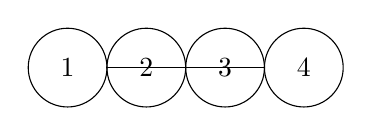
\begin{tikzpicture}
\graph[nodes={circle, draw, minimum size=1cm}] {
  1 -- 2 -- 3 -- 4 -- 1;
};
\end{tikzpicture}
\caption{A simple 4-vertex cycle graph}
\end{figure}

Initial configuration: $c = (2, 1, 1, 0)$\\
Degrees: $\deg = (2, 2, 2, 2)$\\
Active vertices: $\{v_1\}$ since $c_1 = 2 \geq \deg(v_1) = 2$\\
After firing $v_1$: $c' = (0, 2, 1, 1)$\\
Active vertices: $\{v_2\}$\\
After firing $v_2$: $c'' = (1, 0, 2, 1)$\\
And so on...

\end{document}